\documentclass{beamer}

% {{{ beamer stuffs
\setbeamertemplate{footline}[frame number]
\beamertemplatenavigationsymbolsempty%
\logo{
\includegraphics[height=4mm]{fig/LogoEnseeiht.png}}
\usetheme{Montpellier}
\usecolortheme{dolphin}
% }}}

\usepackage{fontspec}
\usepackage{hyperref}
\usepackage{pdflscape}

\usepackage{tikz}
\usetikzlibrary{shapes}

\title{CRAPS Kernel}
\subtitle{Final presentation}
\author{
       Maxime Arthaud
  \and Korantin Auguste
  \and Martin Carton
  \and Étienne Lebrun
}
\titlegraphic{
\includegraphics[width=0.5\textwidth]{fig/LogoEnseeiht.png}}
\date{March 13, 2015}

\begin{document}
  \begin{frame}[plain]
    \titlepage%
  \end{frame}

  \begin{frame}[plain]
    \tableofcontents
  \end{frame}

  \section{The project}
    \begin{frame}{Presentation}
      \begin{itemize}
        \item Implement a basic operating system on CRAPS:
          \begin{itemize}
            \item processor architecture developed by Jean-Christophe
              Buisson for first year students
            \item runs on a Nexys2 board
          \end{itemize}
        \item Goal: make a operating system course
          \begin{itemize}
            \item based on what student know
            \item adding a continuity in courses
          \end{itemize}
      \end{itemize}
    \end{frame}

    \begin{frame}[plain]
      \begin{figure}
        \centering
        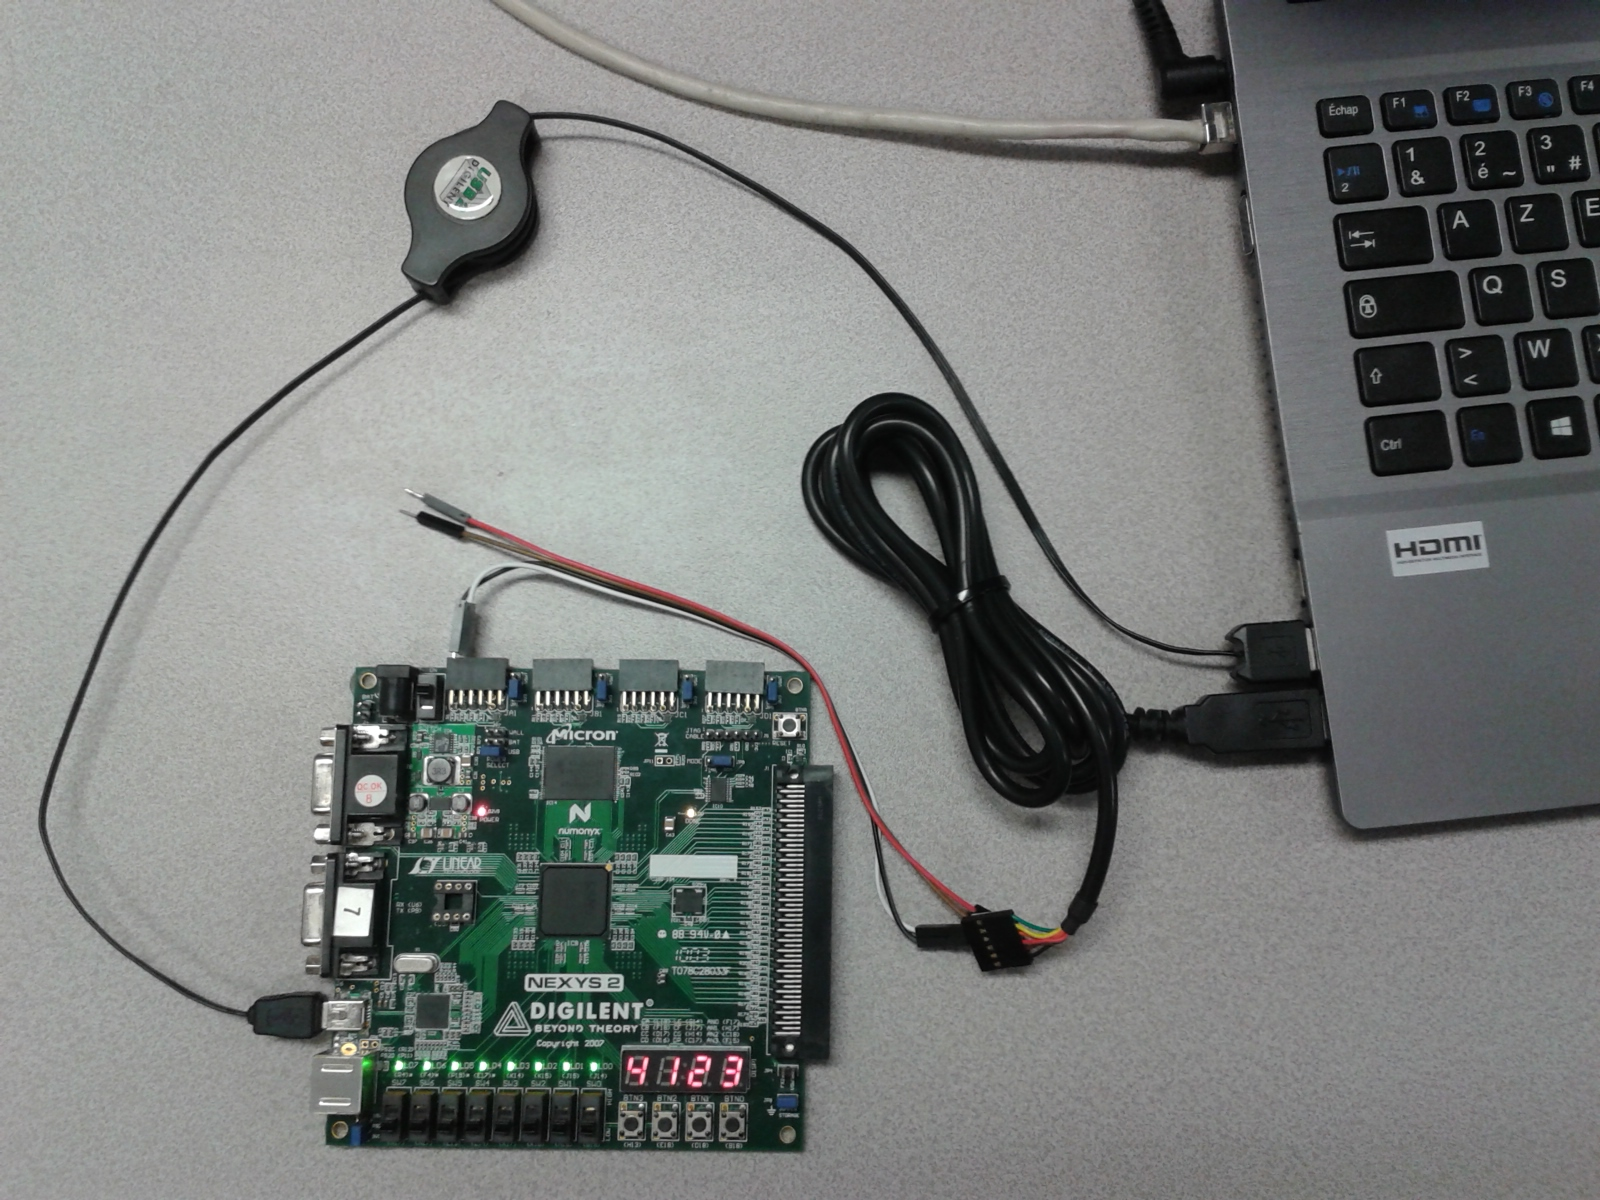
\includegraphics[width=\textwidth, keepaspectratio]{fig/Nexys2.jpg}
        \caption{A Nexys2 board}
      \end{figure}
    \end{frame}

    \begin{frame}{Goal}
      It should show students how a basic operating system works:
        \begin{itemize}
          \item scheduling
          \item interrupts
          \item communications
          \item memory management
        \end{itemize}
    \end{frame}

  \section{Project Management}
    \subsection{Team}
      \begin{frame}{Team Organization}
        \begin{itemize}
          \item Korantin Auguste as \textit{developer}
          \item Maxime Arthaud as \textit{tester}
          \item Martin Carton as \textit{project leader}
          \item Étienne Lebrun as \textit{quality manager}
        \end{itemize}
      \end{frame}

      \begin{frame}{Team Management}
        Quite free, working on what we like, when we like.

        \pause
        \begin{figure}
          \centering
          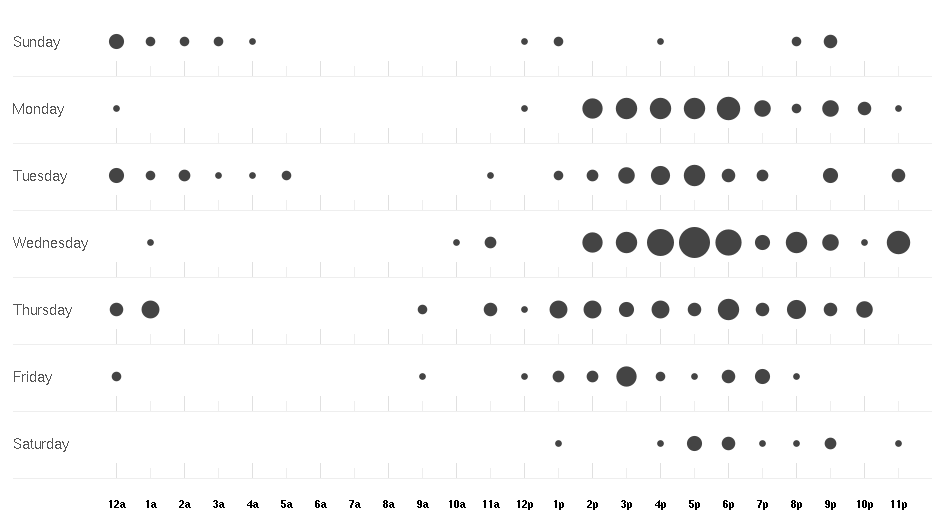
\includegraphics[width=0.9\textwidth]{fig/punchcard.png}
        \end{figure}
      \end{frame}

    \subsection{Project Organization}
      \begin{frame}{Risks Management}
        We have identified three real risks and mitigated them:
        \begin{itemize}
          \item Damaged FPGA
          \item Unable to integrate more RAM
          \item Serial port too slow
        \end{itemize}
      \end{frame}

      \begin{frame}{Actions Management}
        We used a spreadsheet to manage the actions:
          \includegraphics[width=0.9\textwidth,keepaspectratio]
                          {Actions/ActionManagement.pdf}
      \end{frame}

      \begin{frame}{Specifications}
        \begin{itemize}
          \item First week of the project
          \item We identified three main tasks:
            \begin{itemize}
              \item The compiler
              \item The modifications to the processor
              \item The kernel
            \end{itemize}
          \end{itemize}
      \end{frame}

      \begin{frame}{Task Repartition and Planning}
          We used an incremental process, adding features one after another:
          \begin{enumerate}
            \item Write a simple scheduler
            \item Add communications using serial port
            \item Handle dynamic program loading
          \end{enumerate}

          We wrote a planning taking finish-to-start constraints into account.
      \end{frame}

      \begin{frame}[plain]
        \begin{figure}
          \includegraphics[height=\textheight, width=\textwidth, keepaspectratio]
                          {build/Gantt.pdf}
        \end{figure}
      \end{frame}

      \begin{frame}{Test Means}
        Not fully automated because of the constraints of the project:
        \begin{itemize}
          \item hardware: need to manually load test code and test it via the
            monitor
          \item compiler: some automated tests test the compiler itself, but the
            generated code has to be tested manually and it is impossible to be
            exhaustive
          \item kernel: need to use the monitor as well, outputs use 7-segment
            display, switches, etc.
        \end{itemize}

        Creation of a command line tool to load code more easily.
      \end{frame}

      \begin{frame}{Deliverables}
        \begin{itemize}
          \item Documentation and manual for students and teachers
            \begin{itemize}
              \item What we changed
              \item How to use our tools
              \item The syntax of our language
              \item \dots
            \end{itemize}
          \item Kernel, compiler, new processor
          \item Reports, abstracts
        \end{itemize}
      \end{frame}

  \section{Implementation}
    \subsection{Processor Changes}
    \begin{frame}{Extending the Processor}
        Pre-existing version of CRAPS not totally adapted to our needs:
        \begin{itemize}
          \item Not enough memory
          \item No proper interrupts
          \item No external communications
        \end{itemize}
    \end{frame}
    \begin{landscape}
        \begin{frame}[plain]
            \includegraphics[scale=0.22]
                            {build/micromachine_old_fromsvg.pdf}

        \end{frame}
        \begin{frame}[plain]
            \includegraphics[scale=0.22]
                            {build/micromachine_updated_fromsvg.pdf}

        \end{frame}
    \end{landscape}

    \begin{frame}{Adding Memory}
        \begin{itemize}
          \item Extend the RAM module inside the FPGA
          \item Try to use the flash memory
          \item Access the external 16Mb RAM chip
      \end{itemize}
    \end{frame}

    \begin{frame}{Interrupts}
      \begin{itemize}
        \item Add an interrupts module, that keeps the state of each interrupt
        \item Use a priority encoder
        \item The sequencer checks if there is a unhandled interrupt with an
          higher priority that the current execution level
        \item Interrupt table at position 1
      \end{itemize}
    \end{frame}

    \begin{frame}{Other Modifications}
      \begin{itemize}
        \item Add more registers:
          \begin{itemize}
              \item New special purpose register for PIC and new purpose for the
                PSR
              \item Up to 19 general purpose registers can be used be the
                compiler, all 32 registers are now mapped
          \end{itemize}
        \pause
        \item Add a test-and-set instruction
          \begin{itemize}
              \item Working but finally not used
          \end{itemize}
      \end{itemize}
    \end{frame}

    \begin{frame}{Serial Port}
      To communicate with the computer we used a serial port.

      \pause
      We had to modify the processor:
      \begin{itemize}
        \item Add a new built-in module in SHDL
        \item Add a new interrupt in the processor
        \item Map the module to memory
      \end{itemize}

      \pause
      We had some problems:
      \begin{itemize}
        \item the module can cause the synthesis to fail (too complex?)
        \item the communication is slow, we can lose data
      \end{itemize}
    \end{frame}

    \subsection{Compiler}
    \begin{frame}{Compiler}
      \begin{itemize}
        \item Based on the compiler project from the second-year classes.
        \item Language: a (quite large!) subset of C.
        \item Various optimizations.
      \end{itemize}
    \end{frame}

    \begin{frame}{Compiler, in deep}
      \begin{itemize}
        \item Use EGG (Extended Generator Generator), a tool to build an
          attribute grammar
        \item EGG is responsible for the lexical and syntactic analysis
        \item Java for the code generation
      \end{itemize}
    \end{frame}

    \begin{frame}{Compiler optimizations}
      \begin{itemize}
        \item Remove unused functions
        \item Simplify arithmetic expressions
        \item Compute addresses at compile-time
        \item Use optimized instructions
        \item Simplify while(true) loops, if without else block …
      \end{itemize}
    \end{frame}

    \subsection{Kernel}
    \begin{frame}{Scheduler}
      Needed to make ``context switch'': change the current process.

      \begin{columns}
        \begin{column}{0.4\textwidth}
          \begin{figure}
            \centering
            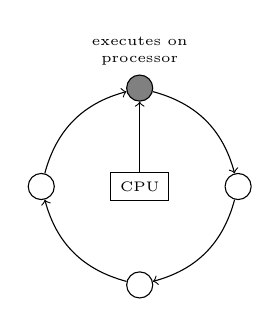
\begin{tikzpicture}[auto, ->, node distance=1.25cm]
              \node[auto] (CPU) [draw, style={font=\tiny}] {CPU};

              \node[auto] (A)   [draw, ellipse, above of=CPU, fill=gray,
              label={[align=center, style={font=\tiny}]executes on\\processor}] {};
              \node[auto] (B)   [draw, ellipse, right of=CPU] {};
              \node[auto] (C)   [draw, ellipse, below of=CPU] {};
              \node[auto] (D)   [draw, ellipse, left  of=CPU] {};

              \path (CPU) edge (A);

              \path (A) edge [bend left] (B);
              \path (B) edge [bend left] (C);
              \path (C) edge [bend left] (D);
              \path (D) edge [bend left] (A);
            \end{tikzpicture}
          \end{figure}
        \end{column}
        \begin{column}{0.6\textwidth}
          \begin{itemize}
            \item Save the current state of the process
            \item Restore the state for the other process
          \end{itemize}

        \end{column}
      \end{columns}

    \end{frame}

    \begin{frame}{Scheduler}
      \begin{itemize}
        \item New interrupt based on the PWM, that will trigger a context switch.
        \item Context switch:
        \begin{enumerate}
           \item Save the registers on the current stack
           \item Change the current stack to the one of the next process
           \item Restore the registers
           \item Return from interrupt (will jump to the address of the
             instruction stored on the stack of the new process)
        \end{enumerate}
      \end{itemize}
    \end{frame}


    \begin{frame}{Memory Management}
      \begin{itemize}
        \item We need to be able to dynamically allocate memory.
        \item In modern computers: virtual memory (segmentation and pagination).
          Too complicated.
        \item We just need three functions: malloc, free, realloc.
        \item How to free all the memory of a process ?
      \end{itemize}
    \end{frame}

    \begin{frame}{Memory Management}
      \begin{itemize}
        \item Stored in blocks, with a header indicating the size and the PID of
          the owner.
        \item All blocks have a size that is a power of two.
        \item We never split/merge/delete blocks, we just reuse them if freed.
        \item We can free all the blocks for a given process.
      \end{itemize}
    \end{frame}

    \begin{frame}[plain]
      \begin{figure}
        \begin{minipage}[c]{0.5\textwidth}
          \caption{Memory layout}
        \end{minipage}\hfill
        \begin{minipage}[c]{0.5\textwidth}
          \includegraphics[height=\textheight]{build/memory_layout_fromsvg.pdf}
        \end{minipage}
      \end{figure}
    \end{frame}

    \subsection{Dynamic Loading}
      \begin{frame}{Dynamic loading}
        \begin{itemize}
          \item Not very hard to do\dots
          \item \dots but we had to make the code position-independent.
        \end{itemize}
      \end{frame}

  \section{Final Result}
    \begin{frame}{Various processes}
      \begin{itemize}
        \item The shell (most important)
        \item Counter
        \item LEDs
        \item \dots and dynamic loading!
      \end{itemize}
    \end{frame}

    \begin{frame}{Demo}
      \begin{itemize}
        \item Compiler
        \item Debugger
        \item Serial console
        \item Process management
      \end{itemize}
    \end{frame}

  \section{Conclusion}
    \begin{frame}{Improvements}
    \end{frame}

    \begin{frame}{Conclusion}
    \end{frame}

  \section{Questions}
    \begin{frame}
      Any questions?
    \end{frame}
\end{document}
